\chapter{Química organometálica: ligação e ligantes}\label{ch:b3:organometallic-bonding}

Em 1951, dois grupos de pesquisa obtiveram, de forma independente, um pó laranja,
estável ao ar, de fórmula $\ce{FeC10H10}$, que não fazia sentido: o ferro não costuma formar
ligações estáveis com o carbono, e certamente não com dois anéis ciclopentadienila ao
mesmo tempo. Em um ano, sua estrutura estava estabelecida: o ferro fica entre dois
anéis paralelos, ligado igualmente aos dez átomos de carbono, um sanduíche. O ferroceno
inaugurou a química organometálica moderna, cujos catalisadores produzem hoje a maior parte dos
polímeros, fármacos e produtos de química fina do mundo (\cref{ch:b3:homogeneous-catalysis}).
Este capítulo explica como os metais se ligam ao monóxido de carbono, às fosfinas, aos alquenos,
aos anéis, aos \omterm{def:b3:organometallic-bonding:carbene}{carbenos} e uns aos outros, e como a \omterm{def:b3:organometallic-bonding:isolobal}{analogia isolobal} liga os
fragmentos organometálicos à química orgânica do carbono.

\begin{recall}
O volume do 1.º ano definiu os compostos organometálicos e usou os reagentes de Grignard.
O volume do 2.º ano introduziu a regra dos 18 elétrons e a contagem de elétrons de valência,
a hapticidade, os ligantes $\pi$-aceptores e $\pi$-doadores com a retrodoação, as etapas
elementares das reações organometálicas (adição oxidativa, eliminação redutiva,
inserção) e os orbitais de fragmento. O \cref{ch:b3:group-theory-applied} contou
os estiramentos CO \omterm{def:b3:group-theory-applied:activity}{ativos no IV} das carbonilas e construiu combinações adaptadas à
simetria; o \cref{ch:b3:complex-spectra-magnetism} relacionou os momentos magnéticos
aos elétrons desemparelhados.
\end{recall}

\begin{omfigure}
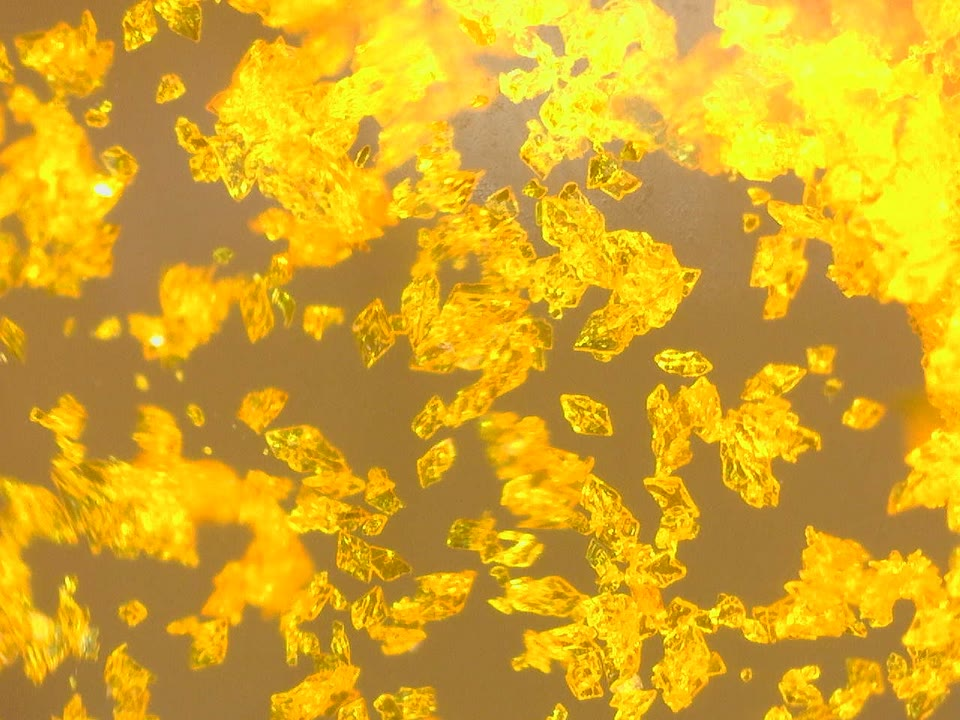
\includegraphics[width=0.5\linewidth]{images/book4/ferrocene-crystals.jpg}

{\small Cristais de ferroceno, $\ce{Fe(C5H5)2}$: um composto organometálico laranja,
estável ao ar, que sublima sob aquecimento brando.}
\end{omfigure}

\section{Contagem de elétrons e estados de oxidação}

\begin{method}[Contar os elétrons, de duas maneiras]\label{met:b3:organometallic-bonding:count}
\begin{enumerate}
  \item Método dos ligantes neutros (covalente): o metal traz um número de elétrons igual ao
        número de seu grupo; cada ligante, tomado neutro, traz 1 (H, \ce{CH3}, Cl, o
        $\eta^1$-alila) ou 2 (CO, \ce{PR3}, alqueno) ou mais ($\eta^5$-\ce{C5H5} 5, $\eta^6$-\ce{C6H6} 6); some um por
        ligação metal--metal e corrija pela carga global.
  \item Método iônico: ligantes como H, \ce{CH3}, Cl, \ce{C5H5} são contados como ânions (2, 2,
        2 e 6 elétrons), e o metal como o cátion $d^n$ resultante; os ligantes neutros,
        como antes.
  \item Os dois dão o mesmo total; o método iônico dá também o estado de oxidação
        e a contagem $d^n$.
\end{enumerate}
\end{method}

\begin{example}[Contagem]\label{ex:b3:organometallic-bonding:count}
$\ce{Fe(CO)5}$: $8 + 5 \times 2 = 18$, ferro(0), $d^8$. Ferroceno: método neutro $8 + 2 \times 5 = 18$; método iônico
$\ce{Fe^{2+}}$ ($d^6$, 6) $+ 2 \times 6$ ($\ce{C5H5-}$) $= 18$, ferro(II). $\ce{Mn2(CO)10}$: cada Mn $7 + 5 \times 2 + 1$ (a ligação
Mn--Mn) $= 18$. Os complexos $d^8$ quadrado-planares como $\ce{[PtCl4]^{2-}}$ ou o catalisador de Wilkinson
$\ce{RhCl(PPh3)3}$ têm 16 elétrons: seu orbital vazio do tipo $p_z$ é alto demais para ser preenchido, e
os complexos quadrado-planares de 16 elétrons são tão estáveis quanto os de 18 elétrons.
\end{example}

\section{Carbonilas e fosfinas}

\begin{definition}[Carbonilas metálicas]\label{def:b3:organometallic-bonding:carbonyl}
Uma \emph{carbonila metálica}\index{carbonila metalica@carbonila metálica} é um complexo com ligantes
monóxido de carbono. Uma \emph{carbonila terminal}\index{carbonila terminal} está ligada a um
só metal pelo carbono; uma \emph{carbonila em ponte}\index{carbonila em ponte} une
dois (ou três) metais.
\end{definition}

Ludwig Mond descobriu em 1890 que o níquel reage com o monóxido de carbono à temperatura
ambiente dando o líquido volátil $\ce{Ni(CO)4}$, que se decompõe de volta em níquel puro
por aquecimento: a base de um processo de refino. O monóxido de carbono se liga aos
metais de transição por seu orbital ocupado mais alto, um par isolado $\sigma$ situado sobretudo
no carbono, e recebe elétrons em seus orbitais $\pi^*$ vazios, também maiores no
carbono.

\begin{definition}[Ligação sinérgica]\label{def:b3:organometallic-bonding:synergic}
A \emph{ligação sinérgica}\index{ligacao sinergica@ligação sinérgica} é o reforço mútuo da
doação $\sigma$ de um ligante para um metal e da retrodoação $\pi$ do metal para o
ligante: a doação torna o metal mais rico em elétrons e mais disposto a devolvê-los,
a retrodoação alivia a carga acumulada pela doação.
\end{definition}

\begin{omfigure}
\begin{tikzpicture}[font=\small, >=Stealth]
  % sigma donation
  \fill[black!70] (0,0) circle (0.14); \node[anchor=north] at (0,-0.4) {M};
  \pic at (0,0) {omlobe={-0.7}{180}};
  \pic at (0,0) {omlobe={0.9}{0}};
  \node[circle, fill=black!40, inner sep=1.6pt] at (1.9,0) {};
  \node[circle, fill=omThm!70, inner sep=1.6pt] at (3.0,0) {};
  \pic at (1.9,0) {omlobe={0.85}{180}};
  \node[font=\scriptsize, anchor=north] at (1.9,-0.25) {C};
  \node[font=\scriptsize, anchor=north] at (3.0,-0.25) {O};
  \draw[->, thick, omThm] (1.4,0.55) to[bend right=30] (0.6,0.55);
  \node[anchor=north] at (1.5,-1.55) {doação $\sigma$};
  % pi back-donation
  \begin{scope}[xshift=6.0cm]
    \fill[black!70] (0,0) circle (0.14); \node[anchor=north] at (0,-1.1) {M};
    \pic at (0,0) {omdxz};
    \node[circle, fill=black!40, inner sep=1.6pt] at (1.9,0) {};
    \node[circle, fill=omThm!70, inner sep=1.6pt] at (3.0,0) {};
    \pic at (1.9,0) {omp={0.9}{90}};
    \pic at (3.0,0) {omp={-0.6}{90}};
    \draw[->, thick, omThm] (0.6,1.05) to[bend left=30] (1.6,1.05);
    \node[anchor=north] at (1.5,-1.55) {retrodoação $\pi$};
  \end{scope}
\end{tikzpicture}

{\small \omterm{def:b3:organometallic-bonding:synergic}{Ligação sinérgica} do monóxido de carbono. À esquerda: o par isolado do carbono (orbital
$\sigma$) doa para um orbital vazio do metal de tipo $\sigma$. À direita: um orbital $d$ preenchido
do metal ($d_{xz}$, com seus dois eixos) se sobrepõe ao orbital $\pi^*$ vazio do CO, maior no
carbono, cujos lobos correspondem às suas fases: os elétrons voltam para um orbital que é
antiligante entre C e O.}
\end{omfigure}

\begin{proposition}[Frequências de estiramento CO]\label{prop:b3:organometallic-bonding:co-frequency}
Quanto mais um metal retrodoa para os orbitais $\pi^*$ de um ligante CO, menor o
número de onda de estiramento C--O.
\end{proposition}

\begin{proof}[Argumento]
Os orbitais $\pi^*$ do CO são antiligantes entre C e O: povoá-los enfraquece a
ligação C--O, diminui sua \omterm{def:b3:quantum-model-systems:oscillator}{constante de força} e, portanto, o número de onda de estiramento, que
varia como a raiz quadrada da \omterm{def:b3:quantum-model-systems:oscillator}{constante de força} (\cref{ch:b3:rovibrational-spectroscopy}).
A doação $\sigma$ retira elétrons de um orbital quase não ligante (ligeiramente
antiligante) para C--O, o que por si só elevaria um pouco o número de onda: a
diminuição observada mostra que a retrodoação domina.
\end{proof}

O monóxido de carbono livre tem sua \omterm{def:b3:rovibrational-spectroscopy:anharmonic}{transição fundamental} em $\omega_e - 2\omega_ex_e = \qty{2143}{cm^{-1}}$; as carbonilas
terminais de complexos neutros absorvem aproximadamente entre 1900 e \qty{2100}{cm^{-1}},
as \omterm{def:b3:organometallic-bonding:carbonyl}{carbonilas em ponte} ainda mais abaixo. Ao longo de uma série isoeletrônica, uma carbonila
aniônica absorve em número de onda menor que a neutra, uma catiônica em número
maior: quanto mais rico em elétrons o metal, mais ele retrodoa. O número de
bandas, pela simetria (\cref{ch:b3:group-theory-applied}), dá a geometria.
% ledger: diat:CO.we, diat:CO.wexe

\begin{proposition}[Interações $\pi$ e desdobramento do campo ligante]\label{prop:b3:organometallic-bonding:pi-delta}
Em um complexo octaédrico, os ligantes $\pi$-aceptores aumentam $\Delta_{\mathrm o}$ e os ligantes $\pi$-doadores
o diminuem.
\end{proposition}

\begin{proof}
Os orbitais $e_g$ só têm simetria $\sigma$. Os orbitais $t_{2g}$ ($d_{xy}$, $d_{xz}$, $d_{yz}$) correspondem a uma combinação $t_{2g}$
dos orbitais $\pi$ dos ligantes: para $d_{xy}$, os quatro ligantes do plano $xy$ oferecem cada um
um orbital $\pi$ perpendicular a seu eixo M--L nesse plano, e a
combinação com sinais alternados tem a simetria de $d_{xy}$ (as demais
combinações se transformam como $t_{1g}$, $t_{1u}$ e $t_{2u}$ e não encontram parceiro $d$). Dois orbitais de
mesma simetria se misturam e se repelem: o mais baixo é empurrado para baixo, o mais alto para cima. Um
$\pi$-aceptor oferece orbitais vazios acima do conjunto $t_{2g}$, que é empurrado para baixo: $\Delta_{\mathrm o}$
aumenta. Um $\pi$-doador oferece orbitais preenchidos abaixo dele, que o empurram para cima: $\Delta_{\mathrm o}$
diminui. O nível $e_g$ não é afetado em nenhum dos dois casos.
\end{proof}

É por isso que CO e \ce{CN-} ficam na extremidade forte da série espectroquímica, e os
haletos e o hidróxido na extremidade fraca, como afirmava o volume do 2.º ano.

\begin{definition}[Parâmetros de Tolman]\label{def:b3:organometallic-bonding:tolman}
O \emph{ângulo de cone de Tolman}\index{angulo de cone de Tolman@ângulo de cone de Tolman} de uma fosfina é o ângulo
no vértice do cone, centrado no metal a uma distância padrão, que envolve exatamente
as superfícies de van der Waals de seus substituintes: uma medida de seu tamanho.
O \emph{parâmetro eletrônico de Tolman}\index{parametro eletronico de Tolman@parâmetro eletrônico de Tolman} é o
número de onda do estiramento CO simétrico de $\ce{Ni(CO)3L}$: quanto mais fortemente a
fosfina L doa, menor ele é.
\end{definition}

As fosfinas são ajustadas de modo independente em tamanho e em doação eletrônica por seus
substituintes: as trialquilfosfinas são doadoras mais fortes que as triarilfosfinas,
e os fosfitos, as mais fracas; $\ce{P(tBu)3}$ é muito mais volumosa que $\ce{PMe3}$. As fosfinas volumosas favorecem
números de coordenação baixos e a dissociação rápida de ligantes, e é por isso que
aparecem em tantos catalisadores.

\section{Ligantes $\pi$}

\begin{definition}[Modelo de Dewar--Chatt--Duncanson]\label{def:b3:organometallic-bonding:dcd}
O \emph{modelo de Dewar--Chatt--Duncanson}\index{modelo de Dewar--Chatt--Duncanson} da
ligação de um alqueno a um metal combina a doação $\sigma$ do orbital $\pi$ C=C
para um orbital vazio do metal com a retrodoação de um orbital $d$ preenchido do metal para
o orbital $\pi^*$ C=C. Seu limite de retrodoação forte é um
\emph{metalaciclopropano}\index{metalaciclopropano}, um anel de três membros
com duas ligações $\sigma$ M--C e uma ligação simples C--C.
\end{definition}

\begin{proposition}[Consequências da retrodoação para um alqueno]\label{prop:b3:organometallic-bonding:dcd}
A coordenação alonga a ligação C=C e dobra os substituintes para trás, para longe do
metal, tanto mais quanto maior a retrodoação.
\end{proposition}

\begin{proof}[Argumento]
Retirar elétrons do orbital $\pi$ (ligante) e acrescentá-los ao orbital $\pi^*$
(antiligante) diminui, nos dois casos, a ordem de ligação C--C. Misturar caráter $\pi^*$
re-hibridiza os carbonos em direção a $sp^3$, cujas ligações com os substituintes apontam para longe
do metal, em direção à geometria do \omterm{def:b3:organometallic-bonding:dcd}{metalaciclopropano}.
\end{proof}

\begin{omfigure}
\begin{tikzpicture}[font=\small, >=Stealth]
  \fill[black!70] (0,0) circle (0.14); \node[anchor=north] at (0,-1.1) {M};
  \pic at (0,0) {omlobe={0.9}{0}};
  \foreach \y in {0.45,-0.45}{\node[circle, fill=black!40, inner sep=1.6pt] at (1.9,\y) {};}
  \pic at (1.9,0.45) {omp={-0.75}{0}};
  \pic at (1.9,-0.45) {omp={-0.75}{0}};
  \draw[->, thick, omThm] (1.3,1.0) to[bend right=30] (0.5,0.6);
  \node[anchor=north] at (1.2,-1.4) {$\sigma$: $\pi$(C=C) $\to$ M};
  \begin{scope}[xshift=5.6cm]
    \fill[black!70] (0,0) circle (0.14); \node[anchor=north] at (0,-1.1) {M};
    \pic at (0,0) {omdxy};
    \foreach \y in {0.45,-0.45}{\node[circle, fill=black!40, inner sep=1.6pt] at (1.9,\y) {};}
    \pic at (1.9,0.45) {omp={-0.75}{0}};
    \pic at (1.9,-0.45) {omp={0.75}{0}};
    \draw[->, thick, omThm] (0.7,0.9) to[bend left=30] (1.5,0.9);
    \node[anchor=north] at (1.2,-1.4) {$\pi$: M $\to$ $\pi^*$(C=C)};
  \end{scope}
\end{tikzpicture}

{\small O \omterm{def:b3:organometallic-bonding:dcd}{modelo de Dewar--Chatt--Duncanson} de um alqueno ligado lateralmente (C=C
vertical, o metal à esquerda). À esquerda: o orbital $\pi$ preenchido (dois orbitais $p$ em
fase) doa para um orbital vazio do metal. À direita: um orbital $d$ preenchido do metal,
de fases correspondentes, doa para o orbital $\pi^*$ vazio (os dois orbitais $p$ fora de
fase).}
\end{omfigure}

O sal de Zeise, $\ce{K[PtCl3(C2H4)]}$, preparado em 1827, foi o primeiro composto organometálico
de um metal de transição; seu eteno fica perpendicular ao plano \ce{PtCl3}, como
o modelo prevê. A alila ($\eta^3$), os dienos ($\eta^4$), os arenos ($\eta^6$) e o anel
ciclopentadienila ($\eta^5$) se ligam da mesma maneira, por vários carbonos ao mesmo tempo.

\begin{definition}[Metalocenos]\label{def:b3:organometallic-bonding:metallocene}
Um \emph{composto sanduíche}\index{composto sanduiche@composto sanduíche} tem um metal entre dois
ligantes anelares planos e paralelos, ligados por todos os seus carbonos; um
\emph{metaloceno}\index{metaloceno} é um composto sanduíche com dois anéis
$\eta^5$-ciclopentadienila, $\ce{M(C5H5)2}$.
\end{definition}

\begin{proposition}[Os orbitais de fronteira do ferroceno]\label{prop:b3:organometallic-bonding:ferrocene}
Em um \omterm{def:b3:organometallic-bonding:metallocene}{metaloceno} de anéis paralelos ($D_{5d}$), os orbitais $d$ do metal se desdobram em $e_{2g}$
($d_{xy}$, $d_{x^2-y^2}$) e $a_{1g}$ ($d_{z^2}$), quase não ligantes e próximos, e $e_{1g}^\ast$ ($d_{xz}$,
$d_{yz}$), fortemente antiligantes; o ferroceno, com seis elétrons $d$ em $e_{2g}^4a_{1g}^2$, tem 18
elétrons e nenhum elétron desemparelhado.
\end{proposition}

\begin{proof}[Argumento]
Os orbitais $\pi$ dos dois anéis se combinam em pares adaptados à simetria $a_{1g}$, $a_{2u}$,
$e_{1g}$, $e_{1u}$, $e_{2g}$, $e_{2u}$ (a partir dos cinco orbitais $\pi$ de cada anel, com zero, um e dois
planos nodais passando pelo eixo). A combinação $e_{1g}$ preenchida dos anéis se sobrepõe
fortemente a $d_{xz}$, $d_{yz}$ (um plano nodal passando pelo eixo cada um): formam-se orbitais
ligantes, sobretudo dos anéis, e antiligantes $e_{1g}^\ast$, sobretudo do metal, empurrados para cima. $d_{xy}$, $d_{x^2-y^2}$
(dois planos nodais) só encontram os orbitais $e_{2g}$ vazios dos anéis e são levemente
estabilizados por retrodoação; $d_{z^2}$ aponta para o buraco no meio de cada anel e
quase não se sobrepõe. Seis elétrons preenchem $e_{2g}$ e $a_{1g}$; com os doze elétrons das
combinações ligantes dos anéis, a contagem é 18.
\end{proof}

\begin{omfigure}
\begin{tikzpicture}[font=\small]
  % sandwich drawing
  \begin{scope}[xshift=-1.0cm]
    \draw[thick, fill=black!8] (0,1.0) ellipse (1.0 and 0.3);
    \draw[thick, fill=black!8] (0,-1.0) ellipse (1.0 and 0.3);
    \foreach \a in {90,162,234,306,18}{\fill[black!60] ({cos(\a)},{1.0+0.3*sin(\a)}) circle (0.07);
      \fill[black!60] ({cos(\a)},{-1.0+0.3*sin(\a)}) circle (0.07);}
    \shade[ball color=orange!70!brown] (0,0) circle (0.2);
    \node[anchor=west] at (0.25,0) {Fe};
  \end{scope}
  % level diagram for four metallocenes
  \pic[transform shape] at (2.1,-0.9) {omlevel={u}{0.5}};
  \pic[transform shape] at (2.7,-0.9) {omlevel={ud}{0.5}};
  \pic[transform shape] at (2.4,-0.4) {omlevel={ud}{0.5}};
  \pic[transform shape] at (2.1,1.0) {omlevel={}{0.5}};
  \pic[transform shape] at (2.7,1.0) {omlevel={}{0.5}};
  \node[anchor=north] at (2.4,-1.3) {\ce{[FeCp2]+}};
  \node[anchor=north, font=\scriptsize] at (2.4,-1.75) {17 e$^-$};
  \pic[transform shape] at (4.3,-0.9) {omlevel={ud}{0.5}};
  \pic[transform shape] at (4.9,-0.9) {omlevel={ud}{0.5}};
  \pic[transform shape] at (4.6,-0.4) {omlevel={ud}{0.5}};
  \pic[transform shape] at (4.3,1.0) {omlevel={}{0.5}};
  \pic[transform shape] at (4.9,1.0) {omlevel={}{0.5}};
  \node[anchor=north] at (4.6,-1.3) {\ce{FeCp2}};
  \node[anchor=north, font=\scriptsize] at (4.6,-1.75) {18 e$^-$};
  \pic[transform shape] at (6.5,-0.9) {omlevel={ud}{0.5}};
  \pic[transform shape] at (7.1,-0.9) {omlevel={ud}{0.5}};
  \pic[transform shape] at (6.8,-0.4) {omlevel={ud}{0.5}};
  \pic[transform shape] at (6.5,1.0) {omlevel={u}{0.5}};
  \pic[transform shape] at (7.1,1.0) {omlevel={}{0.5}};
  \node[anchor=north] at (6.8,-1.3) {\ce{CoCp2}};
  \node[anchor=north, font=\scriptsize] at (6.8,-1.75) {19 e$^-$};
  \pic[transform shape] at (8.7,-0.9) {omlevel={ud}{0.5}};
  \pic[transform shape] at (9.3,-0.9) {omlevel={ud}{0.5}};
  \pic[transform shape] at (9.0,-0.4) {omlevel={ud}{0.5}};
  \pic[transform shape] at (8.7,1.0) {omlevel={u}{0.5}};
  \pic[transform shape] at (9.3,1.0) {omlevel={u}{0.5}};
  \node[anchor=north] at (9.0,-1.3) {\ce{NiCp2}};
  \node[anchor=north, font=\scriptsize] at (9.0,-1.75) {20 e$^-$};
  \node[anchor=east, font=\scriptsize] at (1.8,-0.9) {$e_{2g}$};
  \node[anchor=east, font=\scriptsize] at (1.8,-0.4) {$a_{1g}$};
  \node[anchor=east, font=\scriptsize] at (1.8,1.0) {$e_{1g}^\ast$};
\end{tikzpicture}

{\small À esquerda: a estrutura em sanduíche do ferroceno (anéis eclipsados). À direita: os
orbitais de fronteira de caráter $d$ dos \omterm{def:b3:organometallic-bonding:metallocene}{metalocenos}, $e_{2g}$ e $a_{1g}$ quase não ligantes, $e_{1g}^\ast$
antiligante, preenchidos para o cátion ferrocênio (17 elétrons), o ferroceno (18),
o cobaltoceno (19) e o niqueloceno (20, um elétron em cada orbital $e_{1g}^\ast$, spins
paralelos pela regra de Hund).}
\end{omfigure}

\section{Carbenos, carbinos e ligações metal--metal}

\begin{definition}[Carbenos e complexos de carbeno]\label{def:b3:organometallic-bonding:carbene}
Um \emph{carbeno}\index{carbeno} é uma espécie neutra $\ce{R2C}$ com um carbono divalente
portador de dois elétrons não ligantes. Um \emph{complexo de carbeno}\index{complexo de carbeno}
tem um ligante $\ce{CR2}$ ligado a um metal por uma ligação dupla, $\ce{M=CR2}$. Um complexo de
\emph{carbeno de Fischer}\index{carbeno de Fischer} tem um substituinte heteroatômico
no carbono carbênico e um metal de baixa valência com ligantes $\pi$-aceptores; seu carbono
carbênico é eletrofílico. Um complexo de \emph{carbeno de Schrock}\index{carbeno de Schrock} (alquilideno)
tem apenas substituintes C ou H e um metal do início da série, de valência alta; seu carbono é
nucleofílico. Um \emph{carbeno N-heterocíclico}\index{carbeno N-heterociclico@carbeno N-heterocíclico} é um
carbeno cíclico flanqueado por dois átomos de nitrogênio, estável como composto livre e
ligante $\sigma$-doador forte.
\end{definition}

Os dois tipos de \omterm{def:b3:organometallic-bonding:carbene}{complexos de carbeno} diferem na maneira como a ligação M=C é compartilhada.
Em um \omterm{def:b3:organometallic-bonding:carbene}{carbeno de Fischer}, um \omterm{def:b3:organometallic-bonding:carbene}{carbeno} singleto doa seu par isolado ao metal e
recebe retrodoação em seu orbital $p$ vazio, que o par isolado do heteroátomo
também estabiliza: o carbono continua pobre em elétrons, atacado por nucleófilos. Em um
\omterm{def:b3:organometallic-bonding:carbene}{carbeno de Schrock}, dois fragmentos tripleto, o metal e o \omterm{def:b3:organometallic-bonding:carbene}{carbeno}, formam uma ligação covalente $\sigma +
\pi$, polarizada para o carbono: o alquilideno se comporta como um ilídeo de Wittig.

\begin{definition}[Complexo de carbino]\label{def:b3:organometallic-bonding:carbyne}
Um \emph{complexo de carbino}\index{complexo de carbino} tem uma ligação tripla entre um metal
e um carbono portador de um único substituinte, $\ce{M#CR}$.
\end{definition}

\begin{definition}[Ligação $\delta$, ligação quádrupla]\label{def:b3:organometallic-bonding:delta}
Uma \emph{ligação $\delta$}\index{ligacao delta@ligação $\delta$} é uma ligação cujo orbital tem dois planos nodais
que contêm o eixo internuclear, formada pela sobreposição face a face de dois orbitais $d$
como $d_{xy}$ e $d_{xy}$. Uma \emph{ligação quádrupla}\index{ligacao quadrupla@ligação quádrupla}
combina uma ligação $\sigma$, duas $\pi$ e uma $\delta$ entre dois átomos metálicos.
\end{definition}

\begin{proposition}[{A \omterm{def:b3:organometallic-bonding:delta}{ligação quádrupla} de $[\mathrm{Re_2Cl_8}]^{2-}$}]\label{prop:b3:organometallic-bonding:quadruple}
No $\ce{[Re2Cl8]^{2-}}$ (dois \ce{Re^{III}}, $d^4$ cada), os oito elétrons $d$ ocupam $\sigma^2\pi^4\delta^2$: uma ordem
de ligação 4, que exige o arranjo eclipsado das duas unidades \ce{ReCl4}.
\end{proposition}

\begin{proof}
Com $z$ ao longo do eixo Re--Re e os átomos de Cl ao longo de $\pm x$ e $\pm y$ em cada Re, $d_{x^2-y^2}$
aponta para os cloretos e é usado nas ligações Re--Cl. Os outros quatro orbitais $d$
de cada metal se sobrepõem dois a dois: $d_{z^2}$ com $d_{z^2}$ ao longo do eixo ($\sigma$), $d_{xz}$ com $d_{xz}$ e $d_{yz}$
com $d_{yz}$ lado a lado ($\pi$, duas vezes), $d_{xy}$ com $d_{xy}$ face a face ($\delta$, a mais fraca).
Oito elétrons preenchem as quatro combinações ligantes. Girar uma unidade de $45^\circ$
em torno de $z$ transforma seu $d_{xy}$ em $d_{x^2-y^2}$, que tem sobreposição nula com o outro $d_{xy}$ por
simetria: a ligação $\delta$, e com ela a preferência pela conformação eclipsada, se perde. As
outras três sobreposições têm simetria cilíndrica ou não mudam de magnitude.
\end{proof}

% ledger: geom:Re2Cl8.ReRe
A distância Re--Re de \qty{2.24}{\angstrom} no sal de potássio é muito curta para dois átomos metálicos, e os cloretos das duas metades estão de fato eclipsados, contra
sua repulsão estérica: a ligação $\delta$, por fraca que seja, os mantém ali.

\begin{omfigure}
\tdplotsetmaincoords{58}{25}
\begin{tikzpicture}[tdplot_main_coords, font=\small, scale=1.15]
  \draw[thick, black!60] (0,0,0) -- (0,0,2.0);
  \foreach \z in {0,2.0}{
    \foreach \b in {0,90,180,270}{
      \draw[black!45] (0,0,\z) -- ({1.55*cos(\b)},{1.55*sin(\b)},\z);}
    \foreach \a/\s in {45/omphasepos, 135/omphaseneg, 225/omphasepos, 315/omphaseneg}{
      \path[\s, opacity=0.9] plot[domain=0:360, samples=48, smooth cycle]
        ({0.62*cos(\a)+0.55*cos(\x)*cos(\a)-0.26*sin(\x)*sin(\a)},
         {0.62*sin(\a)+0.55*cos(\x)*sin(\a)+0.26*sin(\x)*cos(\a)}, {\z});}
    \foreach \b in {0,90,180,270}{
      \node[circle, fill=green!45!black, inner sep=1.8pt] at ({1.55*cos(\b)},{1.55*sin(\b)},\z) {};}
    \shade[ball color=black!40] (0,0,\z) circle (0.14);}
  \node[anchor=east, xshift=-1.9cm] at (0,0,2.0) {Re};
  \node[anchor=east, xshift=-1.9cm] at (0,0,0) {Re};
\end{tikzpicture}

{\small A componente $\delta$ da \omterm{def:b3:organometallic-bonding:delta}{ligação quádrupla} de $\ce{[Re2Cl8]^{2-}}$: os orbitais $d_{xy}$ dos
dois átomos de rênio (quatro lobos cada, sinais em azul e laranja) ficam frente a frente
através do eixo Re--Re, lobo sobre lobo de mesmo sinal. Os cloretos (em verde),
eclipsados, ficam ao longo de $x$ e de $y$, entre os lobos.}
\end{omfigure}

\section{A analogia isolobal}

\begin{definition}[Fragmentos isolobais]\label{def:b3:organometallic-bonding:isolobal}
Dois fragmentos moleculares são \emph{isolobais}\index{fragmentos isolobais} quando o
número, a simetria, a energia aproximada e a forma de seus orbitais de fronteira, e o
número de elétrons neles, são semelhantes. A \emph{analogia
isolobal}\index{analogia isolobal} prevê que fragmentos isolobais podem substituir uns aos
outros nas moléculas.
\end{definition}

\begin{proposition}[Séries isolobais]\label{prop:b3:organometallic-bonding:isolobal}
$\ce{CH3}$, $\ce{Mn(CO)5}$ e $\ce{CpFe(CO)2}$ são \omterm{def:b3:organometallic-bonding:isolobal}{isolobais} (um orbital de fronteira, um elétron);
$\ce{CH2}$ e $\ce{Fe(CO)4}$ (dois orbitais, dois elétrons); $\ce{CH}$ e $\ce{Co(CO)3}$ (três orbitais,
três elétrons).
\end{proposition}

\begin{proof}[Argumento]
$\ce{CH3}$ é um fragmento tetraédrico ao qual falta uma ligação: um orbital do tipo $sp^3$ com um
elétron, a um elétron do octeto. $\ce{Mn(CO)5}$ é um octaedro ao qual falta um ligante: o
sítio vazio abriga um orbital híbrido que aponta para fora; com $7 + 10 = 17$ elétrons, ele está a um
elétron de 18, e seu único elétron fica nesse híbrido. Retirar dois ou três
ligantes (ou ligações) dá dois ou três desses orbitais e elétrons, com a
mesma contagem dos dois lados: $\ce{Fe(CO)4}$ tem 16 elétrons ($8 + 8$), a dois de 18;
$\ce{Co(CO)3}$ tem 15 ($9 + 6$), a três.
\end{proof}

\begin{method}[Prever uma estrutura por substituição isolobal]\label{met:b3:organometallic-bonding:isolobal}
\begin{enumerate}
  \item Divida o composto em fragmentos e conte os orbitais de fronteira e os elétrons
        de cada um.
  \item Substitua cada fragmento por seu parceiro \omterm{def:b3:organometallic-bonding:isolobal}{isolobal} orgânico.
  \item O análogo orgânico, se existir, sugere a ligação e a forma:
        $\ce{Mn2(CO)10}$ é o ``etano'', $\ce{Co3(CO)9CH}$ é o ``tetraedrano'' $\ce{(CH)4}$ com três CH
        substituídos por $\ce{Co(CO)3}$.
\end{enumerate}
\end{method}

\begin{omfigure}
\begin{tikzpicture}[font=\small]
  \foreach \y/\l/\r/\n in {0/{\ce{CH3}}/{\ce{Mn(CO)5}}/1, -1.6/{\ce{CH2}}/{\ce{Fe(CO)4}}/2, -3.2/{\ce{CH}}/{\ce{Co(CO)3}}/3}{
    \node at (0,\y) {\l};
    \node at (5.2,\y) {\r};
    \node[font=\large] at (2.6,\y) {$\longleftrightarrow$};
    \node[font=\scriptsize, anchor=south] at (2.6,\y+0.15) {isolobais};
    \node[font=\scriptsize, anchor=west] at (7.0,\y) {\ifnum\n=1 um orbital de fronteira, um elétron\else\ifnum\n=2 dois orbitais de fronteira, dois elétrons\else três orbitais de fronteira, três elétrons\fi\fi};}
  \foreach \a in {0}{\pic at (0.55,0) {omlobe={0.6}{0}};}
  \pic at (6.25,0) {omlobe={0.6}{0}};
  \pic at (0.45,-1.6) {omlobe={0.6}{20}}; \pic at (0.45,-1.6) {omlobe={0.6}{-20}};
  \pic at (6.15,-1.6) {omlobe={0.6}{20}}; \pic at (6.15,-1.6) {omlobe={0.6}{-20}};
  \foreach \t in {-30,0,30}{\pic at (0.4,-3.2) {omlobe={0.55}{\t}}; \pic at (6.1,-3.2) {omlobe={0.55}{\t}};}
\end{tikzpicture}

{\small A série \omterm{def:b3:organometallic-bonding:isolobal}{isolobal} (híbridos de fronteira desenhados esquematicamente): cada fragmento
orgânico e o fragmento \omterm{def:b3:organometallic-bonding:carbonyl}{carbonila metálica} à sua frente têm o mesmo número de
orbitais de fronteira voltados para fora e de elétrons neles, e se combinam de
maneiras análogas.}
\end{omfigure}

\begin{definition}[Interação agóstica]\label{def:b3:organometallic-bonding:agostic}
Uma \emph{interação agóstica}\index{interacao agostica@interação agóstica} é uma ligação de três centros
e dois elétrons entre um metal e uma ligação C--H de um de seus próprios ligantes, na
qual o par ligante C--H doa para um orbital vazio do metal.
\end{definition}

Os hidrogênios agósticos aparecem como distâncias metal--hidrogênio curtas nas estruturas
de difração, como números de onda de estiramento C--H anormalmente baixos e, em RMN, como um
deslocamento para campo alto e um acoplamento $^1J_{\mathrm{CH}}$ reduzido. São instantâneos congelados da
ativação C--H, a primeira etapa de muitas reações catalíticas.

\begin{inthelab}[Trabalhar com carbonilas metálicas]
As \omterm{def:b3:organometallic-bonding:carbonyl}{carbonilas metálicas} são manipuladas em capela com exaustão em funcionamento, sob
nitrogênio ou argônio, sem chama aberta: muitas liberam monóxido de carbono ao serem
aquecidas. As carbonilas voláteis são transferidas por cânula ou em linha de vácuo, nunca
vertidas; os resíduos são destruídos por oxidação lenta (água sanitária ou água de bromo) na
capela. O tetracarbonilníquel, o mais perigoso, não é usado de forma alguma em laboratórios
de ensino.
\end{inthelab}

\begin{safety}{\ghs[0.62cm]{GHS02}\ghs[0.62cm]{GHS06}\ghs[0.62cm]{GHS07}\ghs[0.62cm]{GHS08}\ghs[0.62cm]{GHS09}}
% ledger: ghs4:NiCO4, ghs4:ferrocene
Tetracarbonilníquel: extremamente inflamável, fatal se inalado, suspeito de provocar câncer,
pode prejudicar o feto. Ferroceno: sólido inflamável, nocivo se ingerido;
manipulado como produto de química fina, com luvas e precauções contra poeira.
\end{safety}

\begin{history}[A carbonila de Mond e o sanduíche]
Ludwig Mond e seus colaboradores descobriram o tetracarbonilníquel em 1890 ao
estudar a corrosão de válvulas de níquel pelo monóxido de carbono, e basearam nele um
processo de refino do níquel. O ferroceno foi preparado em 1951 por Thomas Kealy e Peter
Pauson e, de forma independente, por Samuel Miller, John Tebboth e John Tremaine; em 1952,
Geoffrey Wilkinson e Robert Woodward, e Ernst Otto Fischer, propuseram a
estrutura em sanduíche. Fischer e Wilkinson dividiram o Prêmio Nobel de Química de 1973
por seus trabalhos sobre os \omterm{def:b3:organometallic-bonding:metallocene}{compostos sanduíche}.
\end{history}

\section{Exercícios}

\begin{exercise}[$\star$]\label{exo:b3:organometallic-bonding:1}
Conte os elétrons de valência de $\ce{Fe(CO)5}$, $\ce{Mn2(CO)10}$ (por Mn), $\ce{CpMo(CO)3H}$, do ânion de Zeise
$\ce{[PtCl3(C2H4)]-}$, de $\ce{Cr($\eta^6$-C6H6)(CO)3}$ e de $\ce{Cp2ZrCl2}$.
\end{exercise}

\begin{exercise}[$\star$]\label{exo:b3:organometallic-bonding:2}
Dê o estado de oxidação e a contagem $d^n$ do metal em cada composto do
exercício anterior.
\end{exercise}

\begin{exercise}[$\star$]\label{exo:b3:organometallic-bonding:3}
Ordene os números de onda de estiramento CO de $\ce{[V(CO)6]-}$, $\ce{Cr(CO)6}$ e $\ce{[Mn(CO)6]+}$, e justifique.
\end{exercise}

\begin{exercise}[$\star$]\label{exo:b3:organometallic-bonding:4}
Dê os análogos \omterm{def:b3:organometallic-bonding:isolobal}{isolobais} orgânicos de $\ce{Mn2(CO)10}$, $\ce{[CpFe(CO)2]2}$ e $\ce{Co3(CO)9CH}$.
\end{exercise}

\begin{exercise}[$\star\star$]\label{exo:b3:organometallic-bonding:5}
Quantas bandas de estiramento CO $fac$- e $mer$-$\ce{M(CO)3L3}$ apresentam no IV?
\end{exercise}

\begin{exercise}[$\star\star$]\label{exo:b3:organometallic-bonding:6}
Explique por que substituir $\ce{PMe3}$ por $\ce{P(tBu)3}$ em um catalisador pode acelerar uma etapa em que um
ligante precisa deixar o metal.
\end{exercise}

\begin{exercise}[$\star\star$]\label{exo:b3:organometallic-bonding:7}
Classifique $\ce{(CO)5Cr=C(OMe)Ph}$ e $\ce{Ta(=CHCMe3)(CH2CMe3)3}$ como \omterm{def:b3:organometallic-bonding:carbene}{complexos de carbeno} de Fischer ou
de Schrock, e preveja suas reações com uma amina e com uma cetona.
\end{exercise}

\begin{exercise}[$\star\star$]\label{exo:b3:organometallic-bonding:8}
Que ordem de ligação teria um $\ce{[Re2Cl8]^{2-}}$ em conformação alternada? Qual é a ordem de ligação de
$\ce{[Re2Cl8]^{4-}}$, com dois elétrons a mais?
\end{exercise}

\begin{exercise}[$\star\star$]\label{exo:b3:organometallic-bonding:9}
Liste três tipos de evidência de uma \omterm{def:b3:organometallic-bonding:agostic}{interação agóstica} C--H.
\end{exercise}

\begin{exercise}[$\star\star\star$]\label{exo:b3:organometallic-bonding:10}
Dê exemplos de complexos estáveis com 16, 17 e 19 elétrons de valência e explique
cada exceção à regra dos 18 elétrons.
\end{exercise}

\begin{exercise}[$\star\star\star$]\label{exo:b3:organometallic-bonding:11}
$\ce{Cr(CO)6}$ é incolor e diamagnético. Explique, usando o efeito $\pi$-aceptor sobre $\Delta_{\mathrm o}$,
por que ele é de spin baixo e por que suas bandas $d$--$d$ ficam no ultravioleta.
\end{exercise}

\begin{exercise}[$\star\star\star$]\label{exo:b3:organometallic-bonding:12}
A ligação C--C do eteno se alonga de \qty{1.34}{\angstrom} para \qty{1.37}{\angstrom} no sal de Zeise e para
cerca de \qty{1.43}{\angstrom} em um complexo de um metal de baixa valência com retrodoação forte (dados do
exercício). Interprete com o \omterm{def:b3:organometallic-bonding:dcd}{modelo de Dewar--Chatt--Duncanson}.
\end{exercise}

\section{Problema: Sanduíches}

\begin{problem}[{Problema de fim de semana --- sanduíches: contagem de elétrons de quatro
metalocenos, seus orbitais de fronteira e elétrons desemparelhados, sua química redox
e duas questões isolobais e espectroscópicas}]
\label{pb:b3:organometallic-bonding:1}
Os \omterm{def:b3:organometallic-bonding:metallocene}{metalocenos} $\ce{MCp2}$ ($\ce{Cp} = \eta^5$-$\ce{C5H5}$) são conhecidos para M = Fe, Co, Ni e para o cátion ferrocênio.

\medskip\noindent\textbf{Parte I --- Contagem.}
\begin{enumerate}
  \item Conte os elétrons do ferroceno pelo método iônico.
  \item Conte-os pelo método neutro.
  \item Conte os do cobaltoceno.
  \item Conte os do niqueloceno.
  \item Conte os do cátion ferrocênio.
  \item Dê o estado de oxidação e a contagem $d^n$ de cada metal.
\end{enumerate}

\medskip\noindent\textbf{Parte II --- Orbitais e magnetismo.}
\begin{enumerate}[resume]
  \item Classifique os cinco orbitais $d$ em $D_{5d}$.
  \item Quais deles se sobrepõem fortemente aos orbitais $\pi$ dos anéis, e com que
        consequência?
  \item Dê a ordem dos níveis de caráter $d$.
  \item Preencha-os para o ferroceno: elétrons desemparelhados?
  \item Preencha-os para o cobaltoceno: elétrons desemparelhados e \omterm{def:b3:complex-spectra-magnetism:moment}{momento de spin puro}?
  \item Preencha-os para o niqueloceno: elétrons desemparelhados e \omterm{def:b3:complex-spectra-magnetism:moment}{momento de spin puro}?
  \item Preencha-os para o ferrocênio: elétrons desemparelhados? Por que seu momento medido
        fica acima do valor de spin puro?
\end{enumerate}

\medskip\noindent\textbf{Parte III --- Redox.}
\begin{enumerate}[resume]
  \item Por que o cobaltoceno é um redutor forte?
  \item Por que o par ferroceno/ferrocênio é rápido e reversível?
  \item Por que ele é usado como referência interna em eletroquímica não aquosa
        (\cref{ch:b3:electrode-kinetics})?
  \item O que se pode esperar das reações do niqueloceno com ligantes de dois
        elétrons?
\end{enumerate}

\medskip\noindent\textbf{Parte IV --- Fragmentos e espectros.}
\begin{enumerate}[resume]
  \item Mostre que $\ce{CpFe(CO)2}$ é \omterm{def:b3:organometallic-bonding:isolobal}{isolobal} com \ce{CH3} e preveja a estrutura de
        $\ce{[CpFe(CO)2]2}$.
  \item Que dímero misto ele poderia formar com $\ce{Mn(CO)5}$?
  \item Como a substituição de um CO de $\ce{CpMn(CO)3}$ por $\ce{PPh3}$ altera os estiramentos CO
        restantes?
  \item Quantas bandas CO $\ce{Cr($\eta^6$-C6H6)(CO)3}$ ($C_{3v}$) apresenta?
  \item Por que um anel $\eta^5$-Cp pode deslizar para $\eta^3$ durante uma substituição?
  \item Enuncie o resultado: o momento magnético de spin puro do niqueloceno.
\end{enumerate}
\end{problem}
